\documentclass[11pt,reqno]{amsart}

% Page set-up
\usepackage[margin=1.5in]{geometry}
\linespread{1.2}

% Packages
\usepackage{../am221}
\usepackage{bbm}
\usepackage{hyperref}
\usepackage[capitalise,nameinlink]{cleveref}
\hypersetup{colorlinks=true, citecolor=Blue, linkcolor=Brown}

% Commands
\renewcommand{\b}{\mathbf}
\newcommand{\R}{\mathbb{R}}
\newcommand{\one}{\mathbbm{1}}
\newcommand{\E}{\mathbb{E}}

% Thm definitions
\theoremstyle{definition}
\newtheorem{prop}{Proposition}
\theoremstyle{remark}
\newtheorem{rmk}{Remark}

\title{Optimal Transport Problems}
\author{Jiafeng Chen\and Francisco Rivera}
\date{\today}

\begin{document}
\maketitle

\section{Revisions}

By and large, our project goal has remained the same. We have, however, focused
our scope to primarily the Kantorovich optimal transport problem. This is
contrast to the more general but intractable continuous Wassserstein problem.

\section{Theoretical foundations}
The following is a concise review of selected topics in Chapters 2 and 3 in
\cite{peyre2017computational}.

Let $\b a \in \R^m_{\ge 0}$ and $\b b \in \R^n_{\ge 0}$ be two vectors of
non-negative real numbers such that $\b a^T \one = \b b^T \one = 1$, where $a_i$
and $b_j$ represents the amount of ``mass'' at different positions. We are
interested in a matrix $\b P \in \R^{m \times n}_{\ge 0}$ where $P_{ij}$
prescribes the amount of mass flowing from $a_i$ to $b_j$. Naturally, we must
have $\sum_j P_{ij} = a_i$ and $\sum_i P_{ij} = b_j$, so that mass is preserved.
Let $\b C \in \R^{m\times n}$ be a \emph{cost matrix}, where $C_{ij}$ represents
the cost of transporting one unit of $a_i$ to $b_j$. The \emph{Kantorovich
optimal transport problem} is the following linear program:

\begin{align*}
\min_{\b P \in \R^{m \times n}_{\ge 0}} \, & \sum_{i,j} P_{ij} C_{ij} \\
\text{subjected to } & \b P \one = \b a \\
& \b P^T \one = \b b
\end{align*}

\begin{rmk}[A probabilistic view]
Let $X,Y$ be discrete random variables with support $\b x \in \mathcal X^m$ and
$\b y \in \mathcal Y^n$, such that their marginal distributions are prescribed
by $P(X = x_i) = a_i$ and $P(Y = y_j) = b_j$. Let $P_{ij} = P(X = x_i, Y =
y_j)$, making $\b P = (P_{ij})_ {ij}$ a joint distribution. Let $C: \mathcal X
\times \mathcal Y \to \R$ be a cost function. Then the Kantorovich problem is
equivalent to the following:

\[ \min_{\b P}\, \E_{(X,Y) \sim \b P}\bk{C(X,Y)}, \]

where the expectation is taken over valid joint distributions of $(X,Y)$
respecting the marginal distributions. Note that when $\mathcal X = \mathcal Y =
\R^d$ and $C(x,y) = \norm{x-y}^p$, then the optimal value of the above problem
for $X,Y$ is the $p$-Wasserstein distance between the marginal distributions
$\mu_X,\mu_Y$ (up to a power of $1/p$), for discrete, $d$-dimensional
distributions with finite support.
\end{rmk}

It can be shown that the dual problem of the above LP takes the following form:

\begin{align*}
\max_{(\b f, \b g) \in \R^{m} \times \R^n} \, & \sum_i a_i f_i + \sum_j b_j g_j
\\ 
\text{subjected to } & f_i + g_j \le C_{ij}\, \text{ for all $i,j$}.
\end{align*}

The dual problem has a neat economic intuition. Suppose Kevin needs to transport
$\b a$ to $\b b$ but does not understand how. Francisco, his profit-maximizing
colleague, offers him a deal, where Kevin will pay $f_i$ for Francisco to pick
up a unit of mass at $a_i$ and pay $g_j$ for Francisco to dropoff a unit of mass
at $b_j.$ At minimum, Kevin knows that if any $f_i + g_j > C_ {ij}$, then
Francisco is ripping him off, as transporting one unit from $a_i$ to $b_j$ costs
exactly $C_{ij}$. If, on the other hand, $f_i + g_j \le C_{ij}$ is satisfied,
then given any $\b P$, we have

\[
\sum_{i,j} C_{ij}P_{ij} \ge \sum_{i,j} f_i P_{ij} + \sum_{i,j} g_j P_{ij} =
\sum_i f_i a_i + \sum_j g_j b_j \tag{Weak duality},
\]


which means that Kevin cannot lose by taking Francisco's deal. Strong duality,
which indeed holds, here imply that Francisco's optimal profit is zero, and the
trade is fair.

% Note that, fixing $\b f$, the optimal choice of $g_j$ is
% \[ g_j = \min_i (C_{ij} - f_i). \]
% Let $\b g = \b f^{\b C}$ where $(\b f^{\b C})_j = \min_i (C_{ij} - f_i)$,
% which is called a $\b C$-transform of $\b f$; we may reformulate the dual
% problem in terms of only one choice variable $\b f$.

Given optimal solutions to the primal and dual, $\b P$, $(\b f, \b g)$,
respectively, \emph{complementary slackness} implies that

\[ P_{ij} (C_{ij} - f_i - g_j) = 0 \tag{Complementary slackness} \]

holds, which means that $\b P_{ij} \neq 0 \implies C_{ij} = f_i - g_j$ and
vice versa. 
    
\subsection{Dual-ascent algorithms and Hungarian algorithm}

Let $S \subset \{1,\ldots,m\}$ and $S' \subset \{1,\ldots,n\}.$ Let $\one_S$ be
a vector of zeros with ones at location prescribed by $S$. Given $\b f, \b g$ a
feasible pair for the dual, call $(i,j)$ a balanced pair if the condition $f_i +
g_j = C_{ij}$ binds, and inactive otherwise. Then 

\begin{prop}
    Let $(\tilde {\b f}, \tilde {\b g}) = (\b f, \b g) + \epsilon (\one_S,
    -\one_{S'})$. Then $(\tilde {\b f}, \tilde {\b g})$ is dual feasible for a
    sufficiently small $\epsilon$ if for all $i$,
    \[ (i,j) \text{ is balanced } \implies \text{$j \in S'$}. \]
\label{prop:feasible}
\end{prop}

\begin{proof}
    For all $i\in S$, consider
    \[ \epsilon_i = \min_{j: (i,j) \text{ inactive}} C_{ij} - f_i - g_j \]
    Let $\epsilon = \min_i \epsilon_i$. If $(i,j)$ is inactive, then
    \[ \tilde f_i + \tilde g_j \le f_i + \epsilon + g_j\le C_{ij}, \]
    which continues to be inactive. If $(i,j)$ is balanced, then $\tilde f_i +
    \tilde g_j = f_i + g_j = C_{ij}$. In either case, $\tilde {\b f}, \tilde {\b
    g}$ continues to be feasible.
\end{proof}

\begin{prop}
\label{prop:dualascent}
    If a dual feasible solution $(\b f, \b g)$ is not optimal, then there
    exists $S,S'$ such that $(\tilde {\b f}, \tilde {\b g}) = (\b f, \b g) + \epsilon (\one_S,
    -\one_{S'})$ is feasible for small enough $\epsilon$ with a strictly
    better objective.
\end{prop}

\begin{proof}
    Let $\mathcal B$ be the set of balanced edges $(i,j)$, and consider the
    bipartite graph on $\{1,\ldots,m\} \sqcup \{1,\ldots,n\}$ with edges in
    $\mathcal B$. Let there be a source node $s$ with capacitated edges to
    $\{1,\ldots,m\}$ with capacity $a_i$, and a sink node $t$ analogously with
    capacities $b_j$. Consider the maximum flow $\b F$ on the network via
    Ford-Fulkerson. If the throughput of the flow is one, then let $P_ {ij} =
    F_{ij}$, which generates a primal feasible solution $\b P$. Strong duality
    would imply that $\b P, (\b f, \b g)$ are both optimal.
    
    Thus we may assume that the throughput is less than one. We label the nodes
    reached from $s$ where $\b F$ does not saturate capacity, as well as the
    nodes that contribute flow to any labeled nodes. Store the labeled nodes in
    $Q$. Since the graph is bipartite, $Q$ can be split into $S,S'$. Note that
    if $(i,j)$ is balanced and $i\in S$, then $j\in S'$. By Proposition
    \cref{prop:feasible}, $(\tilde {\b f}, \tilde {\b g})$ so defined is
    feasible. We wish to show that
    
    \[ \one_S^T \b a - \one_{S'}^T \b b > 0. \]

    We readily conclude that this is indeed the case by accounting for the
    flow on the network.
\end{proof}

\cref{prop:dualascent} provides a template for the celebrated Hungarian
algorithm \cite{kuhn2010hungarian}. The Hungarian algorithm solves the
Kantorovich problem in the case when both $\b a, \b b \propto \one$. In a
probability context for the Wasserstein distance between empirical measures, if
the measures $\mu, \nu$ are both $d$-dimensional with $n$ observations, the
Hungarian algorithm is $O(n^3)$ for $d>1$ and $O(n\log n)$ for\footnote{In the
$d=1$ case, the optimal transport problem reduces to sorting.} $d = 1$
\cite{bernton2017inference}.

\section{Completed Steps}

We have completed empirical assessments of the LP method as well as the
Hungarian algorithm through computational experiments. The code which implements
this can be found on the
\href{https://github.com/frtennis1/am221-project/tree/master/code}{Github
repository}.\footnote{\url{https://github.com/frtennis1/am221-project/tree/master/code}}

The Hungarian algorithm's runtime can be visualized, along with a log-log plot
regression,

\begin{figure}[h]
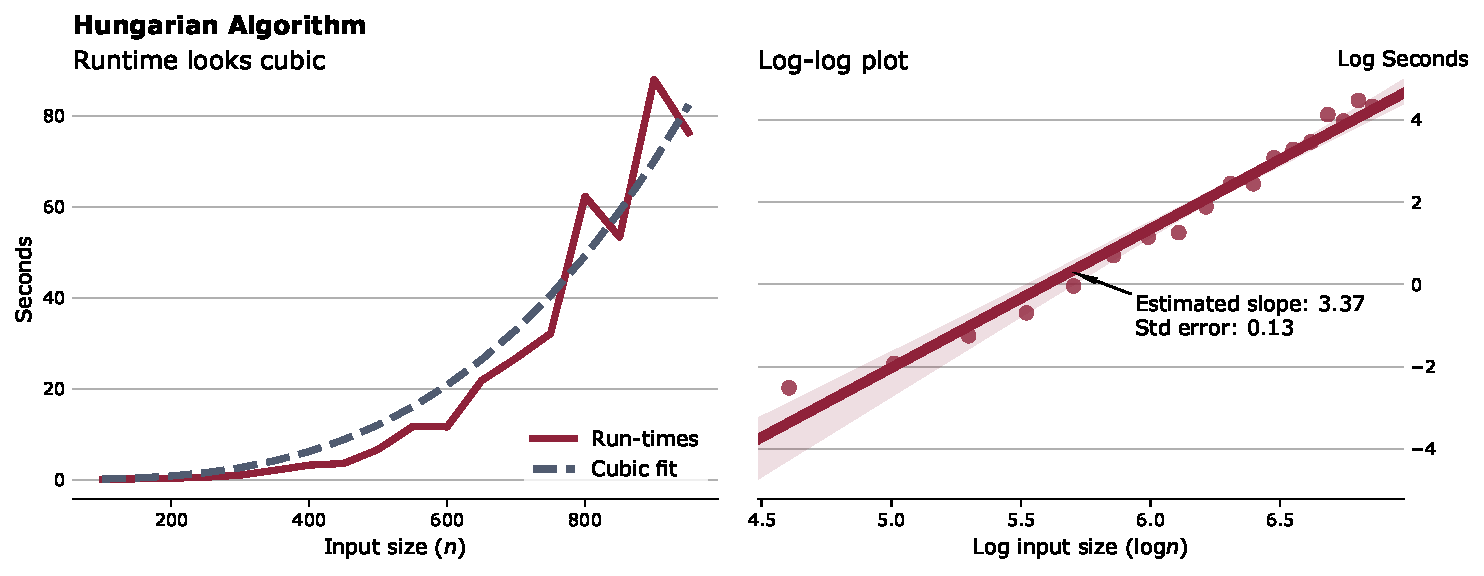
\includegraphics[width=\textwidth]{../../code/hungarianruntime}
\label{fig:hungarianruntime}
\end{figure}


We can also recreate similar plots for the linear-programming algorithm,

\begin{figure}[h]
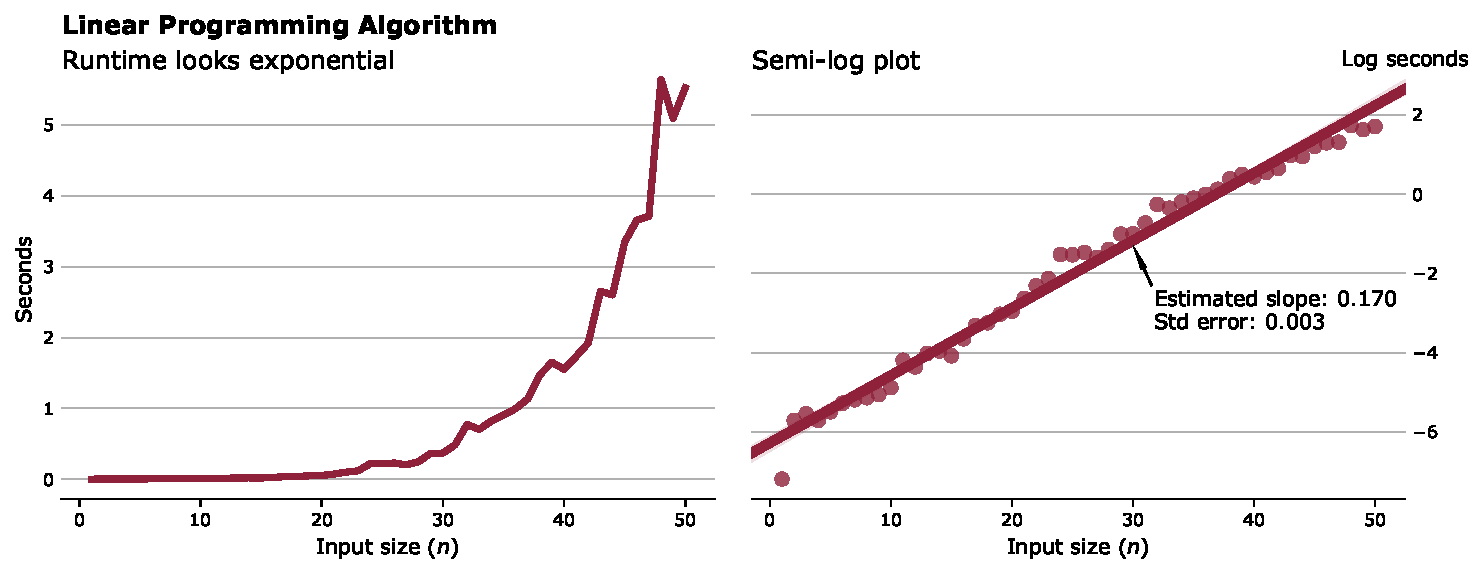
\includegraphics[width=\textwidth]{../../code/lpruntime}
\end{figure}

\section{Next Steps}

The next steps are two-fold. First of all, we will continue our exploration and
analysis of existing algorithms to solve the optimal-transport problem. In
particular, we remain to computationally analyze the dual-ascent algorithms in
generality, and can also explore the auction algorithm. Secondly, we will
attempt to approach the problem from a novel direction, with the ultimate
ambition of arriving at a new algorithm that performs competitively.

% \section{Application value}
 
% \cite{bernton2017inference} is an example of recent work applying the
% Wasserstein distance to statistics and machine learning. 
% Restricting to a subclass of problems called \emph{matching problems},
% where $\b a, \b b \propto \one$.

\bibliographystyle{alpha}
\bibliography{../optimal-transport}
\end{document}
